\section{Crowd plugin development (WP4)}

\paragraph{Generation of the path}~

\noindent The algorithm of least-effort approach is divided in many points.
\begin{itemize}
  \item Grid arrangement and setting up of the grid.
  \item Computation of the minimum on a graph with the $A*$ algorithm.
  \item Computation of the authorised velocity field.
  \item Finding the exclusion zones in order to do the minimisation.
  \item Update of the graph with the attribution of a new weight on the edges: each character affect the weight of its neighbour edges.
\end{itemize}

\todoall{C’est dommage de s’arrêter en si bon chemin. Pour chaque
  itemize une description d’un paraphe pour décrire les efforts et
  avancés menés ne serait pas un luxe. Par exemple pour chaque point on peut se poser la question du comment ? }

\todovl{Ajout screenshot mouvement perso}

\noindent We also started coding the classes that we will use (summarised on Figure \ref{crowd_classes}):
\begin{description}
  \item[Graph] This class describes the graph that was set up, with a set of nodes and a dictionary of dictionaries of edges.
  \item[Individual] This class describe an individual within the crowd. It includes the position, maximal speed, optimal speed, trajectory and some variables to compute the energy of the individual.
  \item[Crowd] contains a set of individuals and the graph.
  \item[Environment] gives the set of forbidden regions.
  \item[Blend*] These are the classes using Blender. They take the corresponding ``non-blend'' class and convert it into a Blender object, usable in Blender. 
\end{description}

We also try to keep as much code as possible independent from Blender. It will lead to easier tests and a more portable code from Blender to another 3D software.

\begin{figure}[h]
  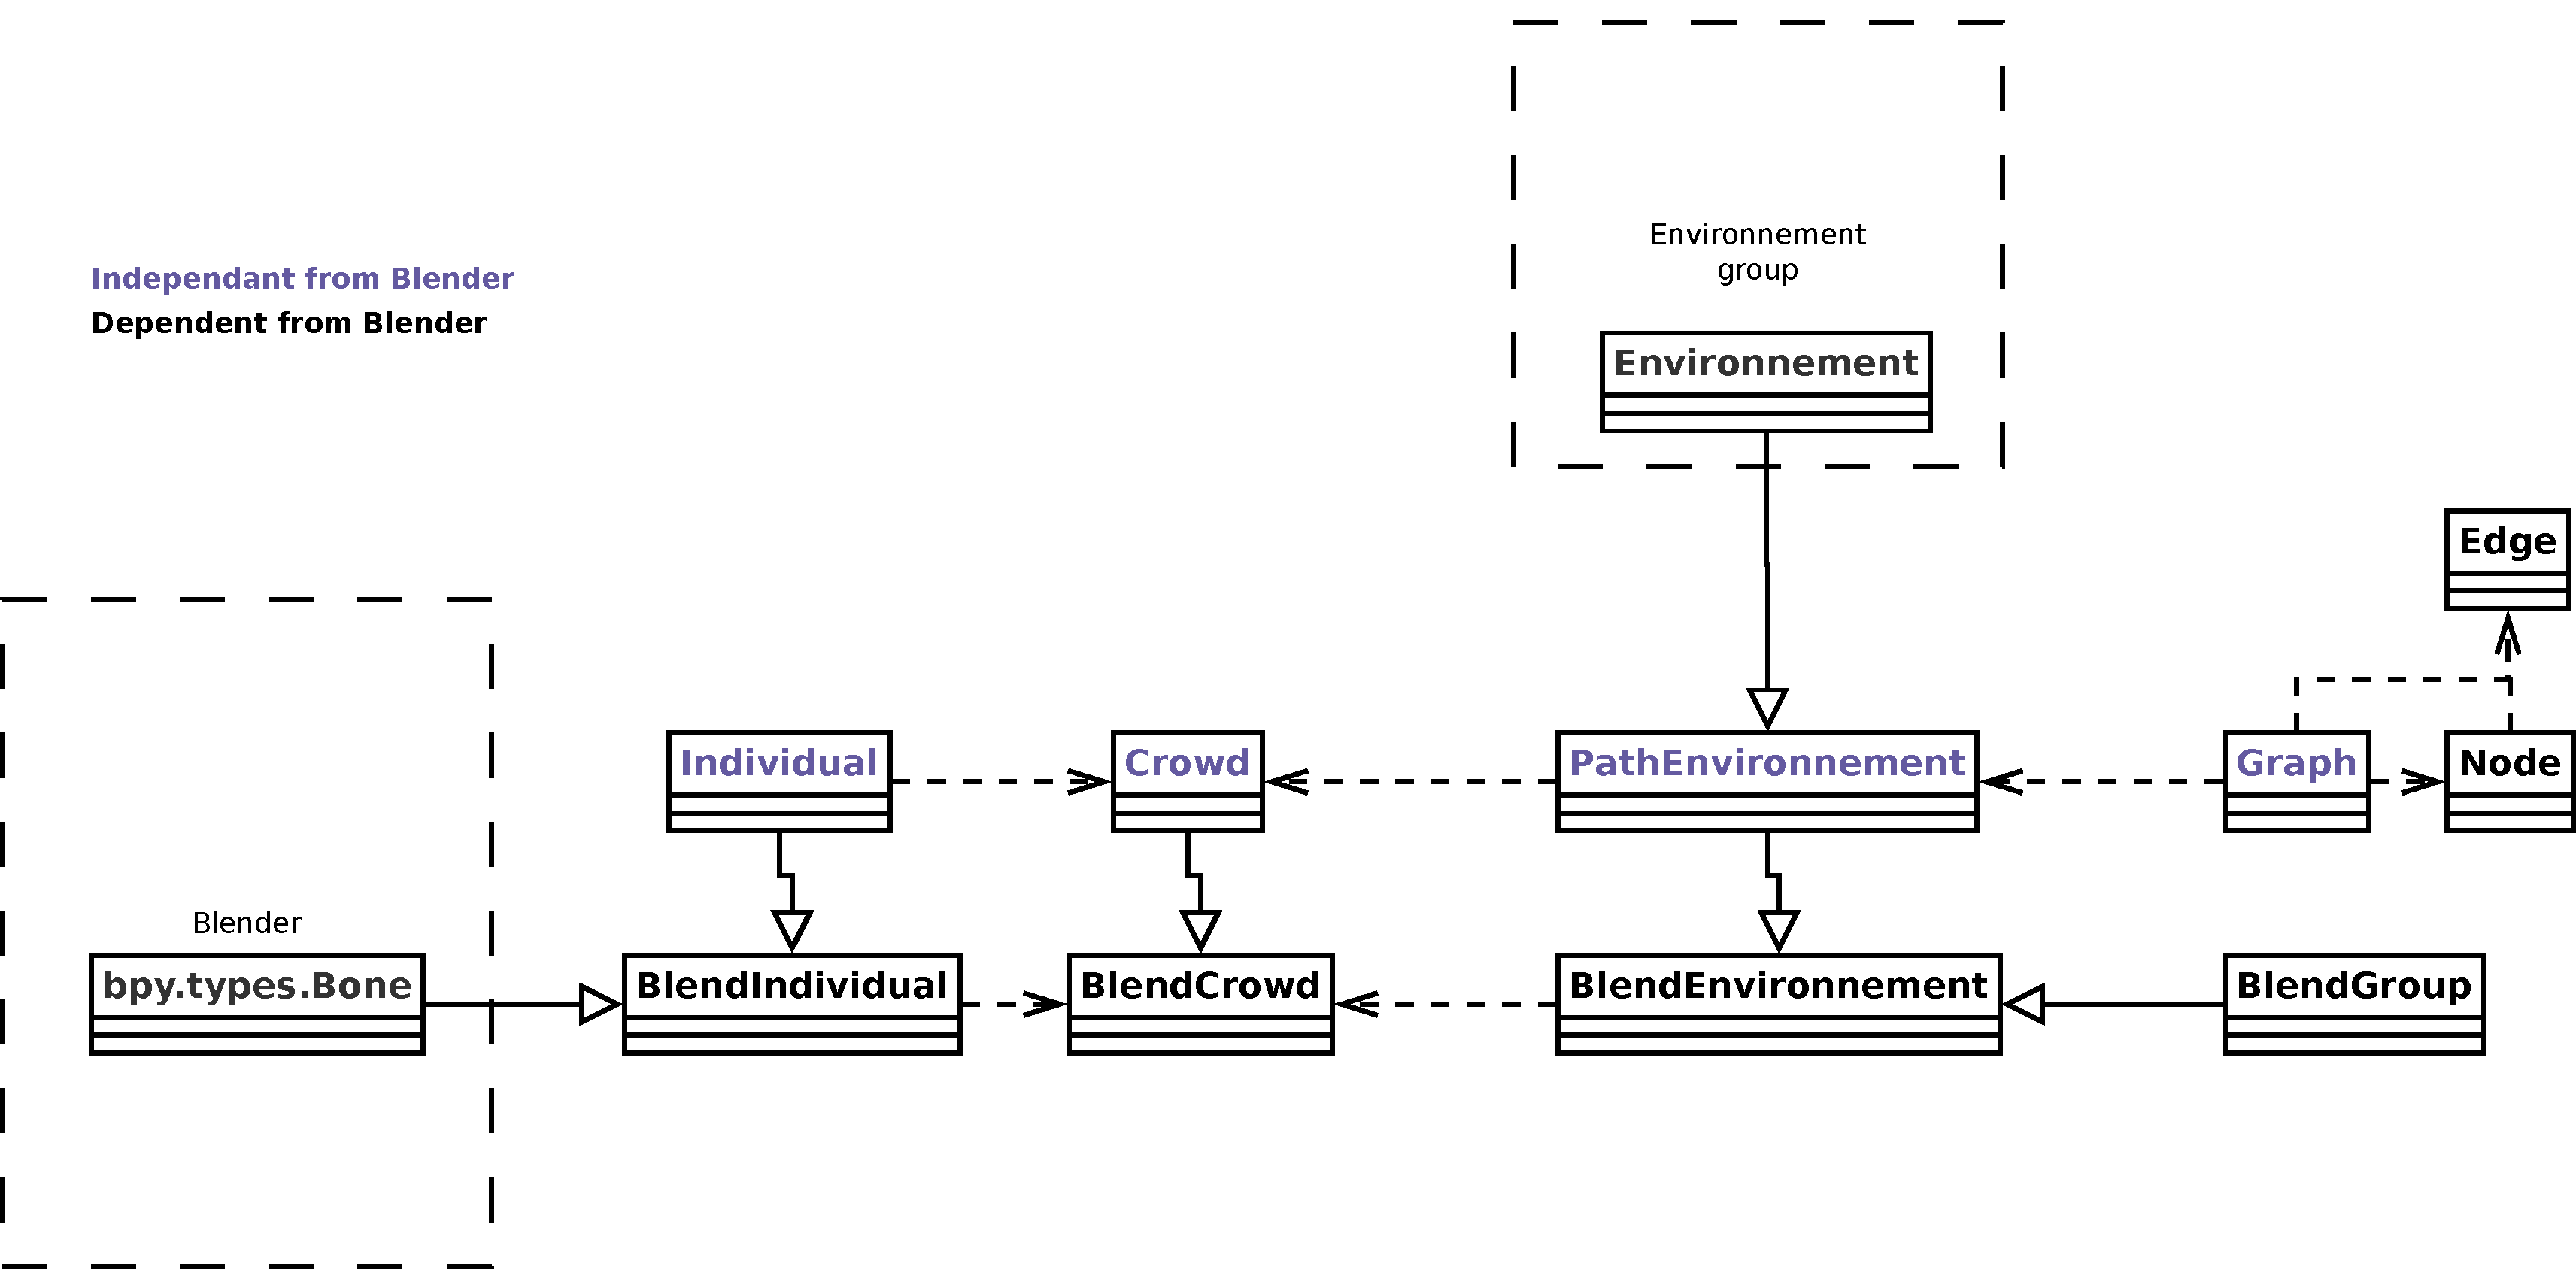
\includegraphics[width=15cm]{crowd_final.pdf}
  \caption{Classes of \texttt{crowd plug-in} and relations between them.}
  \label{crowd_classes}
\end{figure}

\paragraph{Motions of the characters}~

As stated in the paragraph \ref{WP2_motion}, the bibliographical work on the animation of characters was longer than expected and is currently being finalised: the implementation part has yet not begun.



